\documentclass{standalone}
\usepackage[utf8]{inputenc}
\usepackage{tikz}
\usetikzlibrary{positioning}
%\usepackage{pstricks}
\title{Visualization of Morenet}
\author{Xinliang Dai}
\date{March 2020}

\begin{document}
    % original
    \begin{figure}
        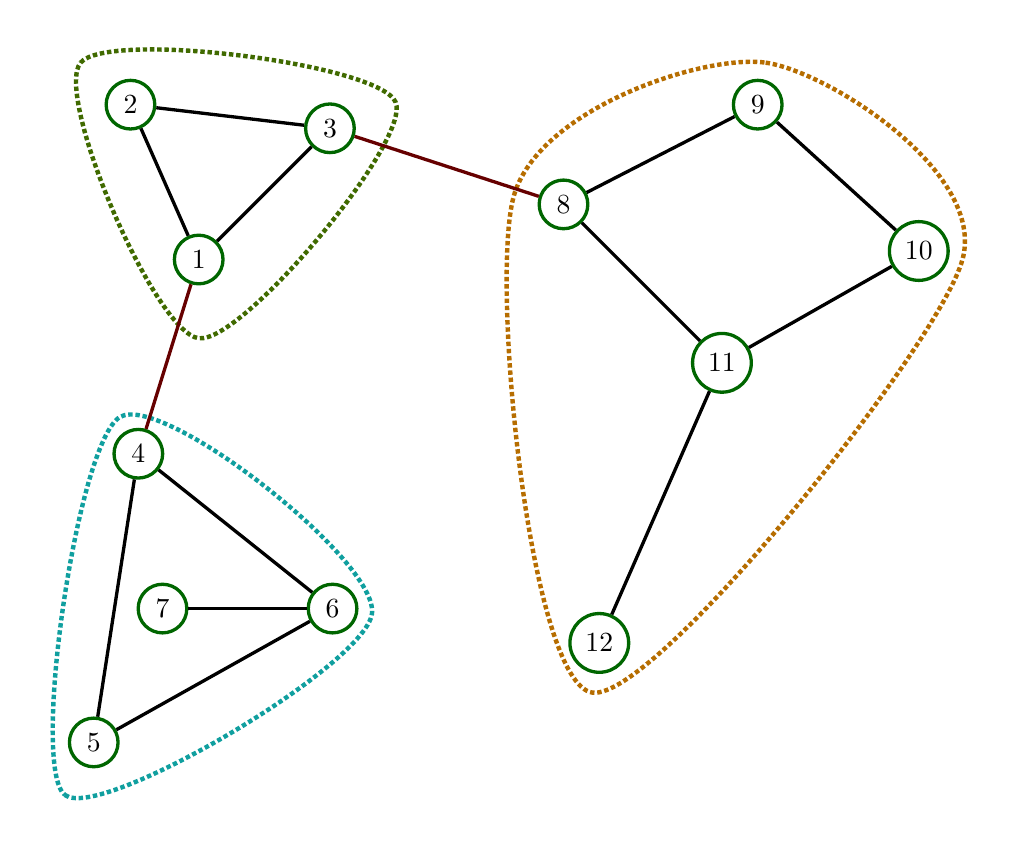
\begin{tikzpicture}[
        core_node/.style={circle, draw=black!60!green, very thick, minimum size=4mm},  %fill=black!15!green,
        copy_node/.style={rectangle, draw=blue!60, fill=blue!5, very thick, minimum size=5mm},
        ]
            % areas
            \draw [color={rgb:red,2;green,4;yellow,1;black,5}, ultra thick,  densely dotted] plot [mark=none, smooth cycle] coordinates {(0,-1)  (-1.5,2.5)  (2.5,2) };
            \draw[color={rgb:red,1;cyan,10;black,5}, ultra thick,  densely dotted] plot [mark=none, smooth cycle] coordinates {(-1,-2)  (-1.7,-6.8)  (2.2,-4.5) };
            \draw[color={rgb:red,4;green,2;yellow,1}, ultra thick,  densely dotted] plot [mark=none, smooth cycle] coordinates {(4,0.8)  (7.2,2.5)  (9.7,0) (5, -5.5)};
        
            % transmission
            \node[core_node]    (core_1)                                               {1};
            \node[core_node]    (core_2)   [above left  = 15mm and 4mm of core_1]      {2};
            \node[core_node]    (core_3)   [above right = 12mm and 12mm of core_1]     {3};
            % distribution 1
            \node[core_node]    (core_4)   [below left  = 20mm and 3mm of core_1]      {4};
            \node[core_node]    (core_5)   [below left  = 32mm and 1mm of core_4]      {5};
            \node[core_node]    (core_6)   [below right = 15mm and 20mm of core_4]     {6};
            \node[core_node]    (core_7)   [left        = 15mm of core_6]              {7};
            % distribution 2
            \node[core_node]    (core_8)   [below right  = 5mm and 25 mm of core_3]    {8};
            \node[core_node]    (core_9)   [above right  = 8mm and 20mm of core_8]     {9};
            \node[core_node]    (core_10)  [below right  = 0.8mm and 40mm of core_8]   {10};
            \node[core_node]    (core_11)  [below right  = 15mm and 15mm of core_8]    {11};
            \node[core_node]    (core_12)  [below left  = 30mm and 10mm of core_11]    {12};
            
            % Lines
            \draw[black, very thick, -] (core_1) -- (core_2);
            \draw[black, very thick, -] (core_2) -- (core_3);
            \draw[black, very thick, -] (core_3) -- (core_1);
            \draw[black, very thick, -] (core_4) -- (core_5);
            \draw[black, very thick, -] (core_5) -- (core_6);
            \draw[black, very thick, -] (core_6) -- (core_7);
            \draw[black, very thick, -] (core_6) -- (core_4);
            \draw[black, very thick, -] (core_8) -- (core_9);
            \draw[black, very thick, -] (core_9) -- (core_10);
            \draw[black, very thick, -] (core_10) -- (core_11);
            \draw[black, very thick, -] (core_11) -- (core_12);
            \draw[black, very thick, -] (core_11) -- (core_8);
            
            % connection
            \draw[color=black!60!red, very thick,-] (core_1) -- (core_4);
            \draw[color=black!60!red, very thick,-] (core_3) -- (core_8);


        \end{tikzpicture}
    \end{figure}

    % transmission's perspective
    \begin{figure}
        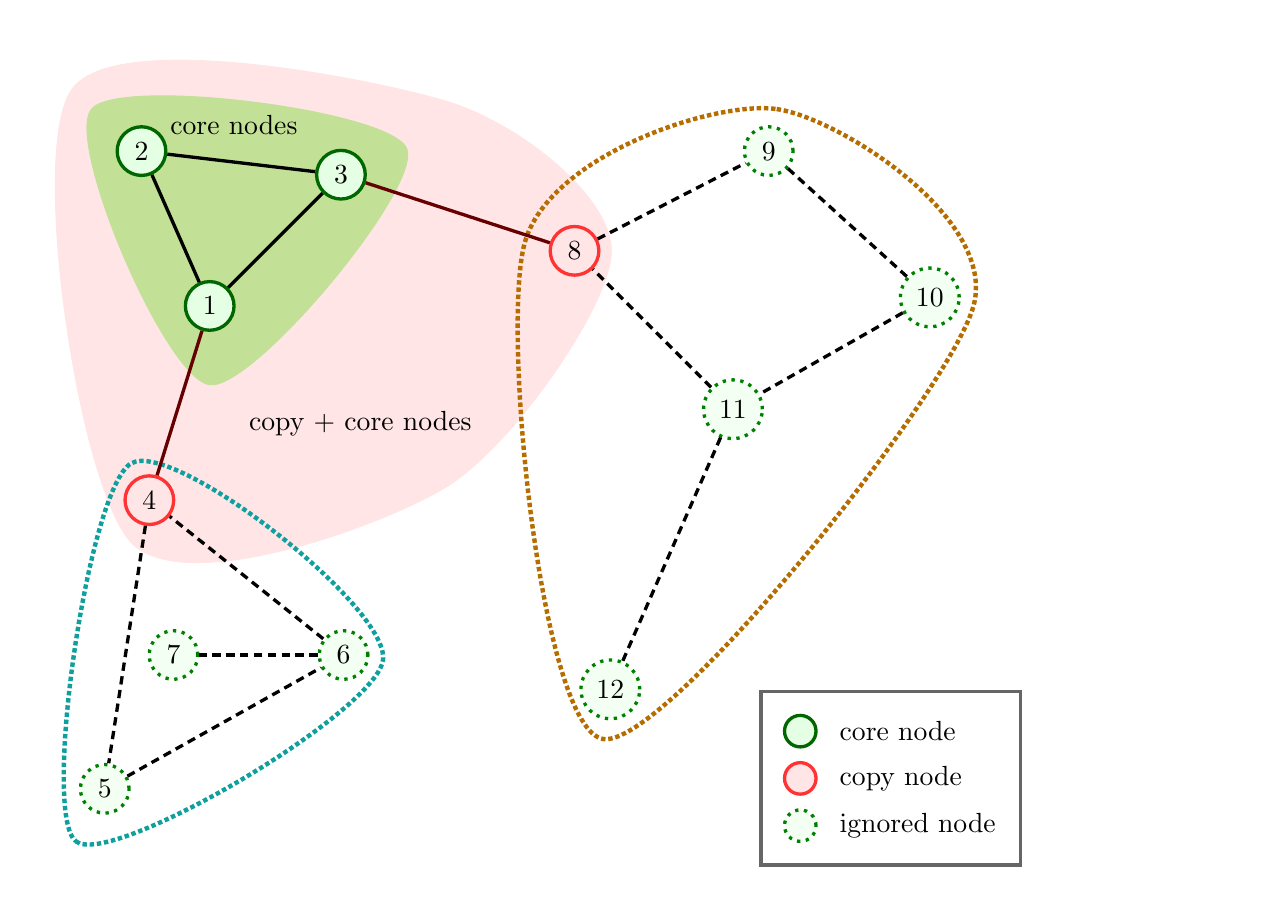
\begin{tikzpicture}[
        core_node/.style={circle, draw=black!60!green, fill=green!10,very thick, minimum size=4mm},
        copy_node/.style={circle, draw=red!80, fill=red!10, very thick, minimum size=4mm},
        core_node_ignore/.style={circle, dotted, draw=black!50!green, fill=green!5,very thick, minimum size=4mm}
        ]
            % Areas
            % rgb:pink,10;green,2;yellow,1
            \filldraw [color=red!10] plot [mark=none, smooth cycle] coordinates { (-1.75,2.75)  (-1,-3) (3, -2.3) (5.1, 0.7) (3, 2.6)};
            \filldraw [color={rgb:red,2;green,4;yellow,1;white,10}] plot [mark=none, smooth cycle] coordinates {(0,-1)  (-1.5,2.5)  (2.5,2) };
            \draw[color={rgb:red,1;cyan,10;black,5}, ultra thick,  densely dotted] plot [mark=none, smooth cycle] coordinates {(-1,-2)  (-1.7,-6.8)  (2.2,-4.5) };
            \draw[color={rgb:red,4;green,2;yellow,1}, ultra thick,  densely dotted] plot [mark=none, smooth cycle] coordinates {(4,0.8)  (7.2,2.5)  (9.7,0) (5, -5.5)};


            % transmission
            \node[core_node]    (core_1)                                               {1};
            \node[core_node]    (core_2)   [above left  = 15mm and 4mm of core_1]      {2};
            \node[core_node]    (core_3)   [above right = 12mm and 12mm of core_1]     {3};
            % distribution 1
            \node[copy_node]    (core_4)   [below left  = 20mm and 3mm of core_1]             {4};
            \node[core_node_ignore]    (core_5)   [below left  = 32mm and 1mm of core_4]      {5};
            \node[core_node_ignore]    (core_6)   [below right = 15mm and 20mm of core_4]     {6};
            \node[core_node_ignore]    (core_7)   [left        = 15mm of core_6]              {7};
            % distribution 2
            \node[copy_node]    (core_8)   [below right  = 5mm and 25 mm of core_3]           {8};
            \node[core_node_ignore]    (core_9)   [above right  = 8mm and 20mm of core_8]     {9};
            \node[core_node_ignore]    (core_10)  [below right  = 0.8mm and 40mm of core_8]   {10};
            \node[core_node_ignore]    (core_11)  [below right  = 15mm and 15mm of core_8]    {11};
            \node[core_node_ignore]    (core_12)  [below left  = 30mm and 10mm of core_11]    {12};
            
            % Lines
            \draw[black, very thick, -] (core_1) -- (core_2);
            \draw[black, very thick, -] (core_2) -- (core_3);
            \draw[black, very thick, -] (core_3) -- (core_1);
            \draw[black, very thick, densely dashed] (core_4) -- (core_5);
            \draw[black, very thick, densely dashed] (core_5) -- (core_6);
            \draw[black, very thick, densely dashed] (core_6) -- (core_7);
            \draw[black, very thick, densely dashed] (core_6) -- (core_4);
            \draw[black, very thick, densely dashed] (core_8) -- (core_9);
            \draw[black, very thick, densely dashed] (core_9) -- (core_10);
            \draw[black, very thick, densely dashed] (core_10) -- (core_11);
            \draw[black, very thick, densely dashed] (core_11) -- (core_12);
            \draw[black, very thick, densely dashed] (core_11) -- (core_8);
            % connection
            \draw[color=black!60!red, very thick,-] (core_1) -- (core_4);
            \draw[color=black!60!red, very thick,-] (core_3) -- (core_8);
            
            % text
            \node[text width=5cm] at (3,-1.5) {copy + core nodes};
            \node[text width=5cm] at (2, 2.3) {core nodes};
            % grid to estimate coordinate
            % \draw[step=1cm,gray,very thin, -] (-2,-8) grid (10,4);
            % legend
            \draw[color = black!60, fill = white, very thick] (7cm,-4.9cm) rectangle (10.3cm,-7.1cm);
            \node[core_node] at (7.5cm,-5.4cm)        { };
            \node[copy_node] at (7.5cm,-6cm)        { };
            \node[core_node_ignore] at (7.5cm,-6.6cm) { };
            \node[text width=5cm] at (10.5cm,-5.4cm) {core node};
            \node[text width=5cm] at (10.5cm, -6cm) {copy node};
            \node[text width=5cm] at (10.5cm, -6.6cm) {ignored node};
        \end{tikzpicture}
    \end{figure}

    % 1st distribution's perspective
    \begin{figure}
        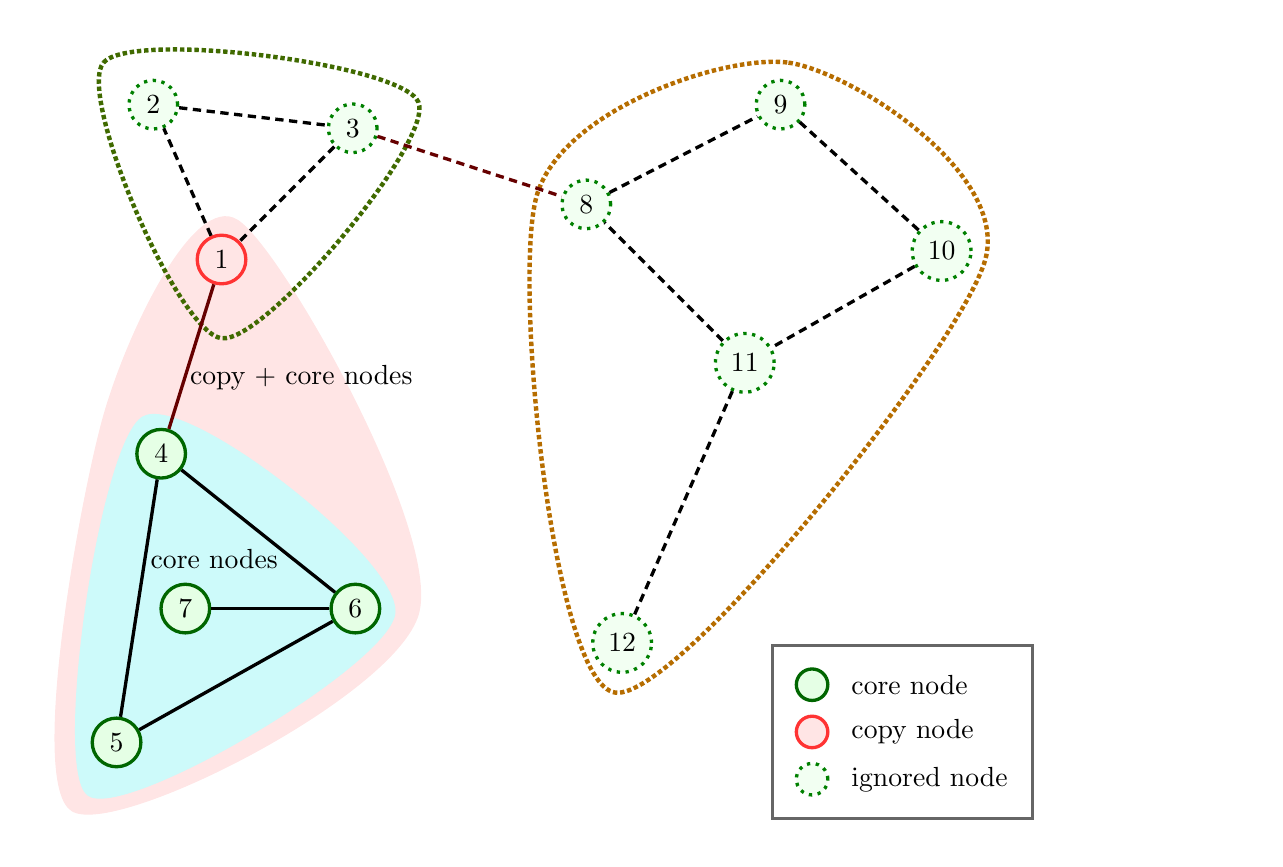
\begin{tikzpicture}[
        core_node/.style={circle, draw=black!60!green, fill=green!10,very thick, minimum size=4mm},
        copy_node/.style={circle, draw=red!80, fill=red!10, very thick, minimum size=4mm},
        core_node_ignore/.style={circle, dotted, draw=black!50!green, fill=green!5,very thick, minimum size=4mm}
        ]
            % Areas
            % rgb:pink,10;green,2;yellow,1
            \filldraw [color=red!10] plot [mark=none, smooth cycle] coordinates { (-1.5,-2)  (-1.9,-7)  (2.5,-4.5) (0.2,0.5)};
            \draw [color={rgb:red,2;green,4;yellow,1;black,5}, ultra thick,  densely dotted] plot [mark=none, smooth cycle] coordinates {(0,-1)  (-1.5,2.5)  (2.5,2) };
            \filldraw[color={rgb:red,1;cyan,10;white,40}] plot [mark=none, smooth cycle] coordinates {(-1,-2)  (-1.7,-6.8)  (2.2,-4.5) };
            \draw[color={rgb:red,4;green,2;yellow,1}, ultra thick,  densely dotted] plot [mark=none, smooth cycle] coordinates {(4,0.8)  (7.2,2.5)  (9.7,0) (5, -5.5)};


            % transmission
            \node[copy_node]    (core_1)                                               {1};
            \node[core_node_ignore]    (core_2)   [above left  = 15mm and 4mm of core_1]      {2};
            \node[core_node_ignore]    (core_3)   [above right = 12mm and 12mm of core_1]     {3};
            % distribution 1
            \node[core_node]    (core_4)   [below left  = 20mm and 3mm of core_1]             {4};
            \node[core_node]    (core_5)   [below left  = 32mm and 1mm of core_4]      {5};
            \node[core_node]    (core_6)   [below right = 15mm and 20mm of core_4]     {6};
            \node[core_node]    (core_7)   [left        = 15mm of core_6]              {7};
            % distribution 2
            \node[core_node_ignore]    (core_8)   [below right  = 5mm and 25 mm of core_3]           {8};
            \node[core_node_ignore]    (core_9)   [above right  = 8mm and 20mm of core_8]     {9};
            \node[core_node_ignore]    (core_10)  [below right  = 0.8mm and 40mm of core_8]   {10};
            \node[core_node_ignore]    (core_11)  [below right  = 15mm and 15mm of core_8]    {11};
            \node[core_node_ignore]    (core_12)  [below left  = 30mm and 10mm of core_11]    {12};
            
            % Lines
            \draw[black, very thick, densely dashed] (core_1) -- (core_2);
            \draw[black, very thick, densely dashed] (core_2) -- (core_3);
            \draw[black, very thick, densely dashed] (core_3) -- (core_1);
            \draw[black, very thick, -] (core_4) -- (core_5);
            \draw[black, very thick, -] (core_5) -- (core_6);
            \draw[black, very thick, -] (core_6) -- (core_7);
            \draw[black, very thick, -] (core_6) -- (core_4);
            \draw[black, very thick, densely dashed] (core_8) -- (core_9);
            \draw[black, very thick, densely dashed] (core_9) -- (core_10);
            \draw[black, very thick, densely dashed] (core_10) -- (core_11);
            \draw[black, very thick, densely dashed] (core_11) -- (core_12);
            \draw[black, very thick, densely dashed] (core_11) -- (core_8);
            % connection
            \draw[color=black!60!red, very thick,-] (core_1) -- (core_4);
            \draw[color=black!60!red, very thick, densely dashed] (core_3) -- (core_8);
            
            % text
            \node[text width=5cm] at (2.1,-1.5) {copy + core nodes};
            \node[text width=5cm] at (1.6, -3.8) {core nodes};
            % grid to estimate coordinate
            % \draw[step=1cm,gray,very thin, -] (-2,-8) grid (10,4);
            % legend
            \draw[color = black!60, fill = white, very thick] (7cm,-4.9cm) rectangle (10.3cm,-7.1cm);
            \node[core_node] at (7.5cm,-5.4cm)        { };
            \node[copy_node] at (7.5cm,-6cm)        { };
            \node[core_node_ignore] at (7.5cm,-6.6cm) { };
            \node[text width=5cm] at (10.5cm,-5.4cm) {core node};
            \node[text width=5cm] at (10.5cm, -6cm) {copy node};
            \node[text width=5cm] at (10.5cm, -6.6cm) {ignored node};
        \end{tikzpicture}
    \end{figure}

    % 2nd distribution's perspective
    \begin{figure}
        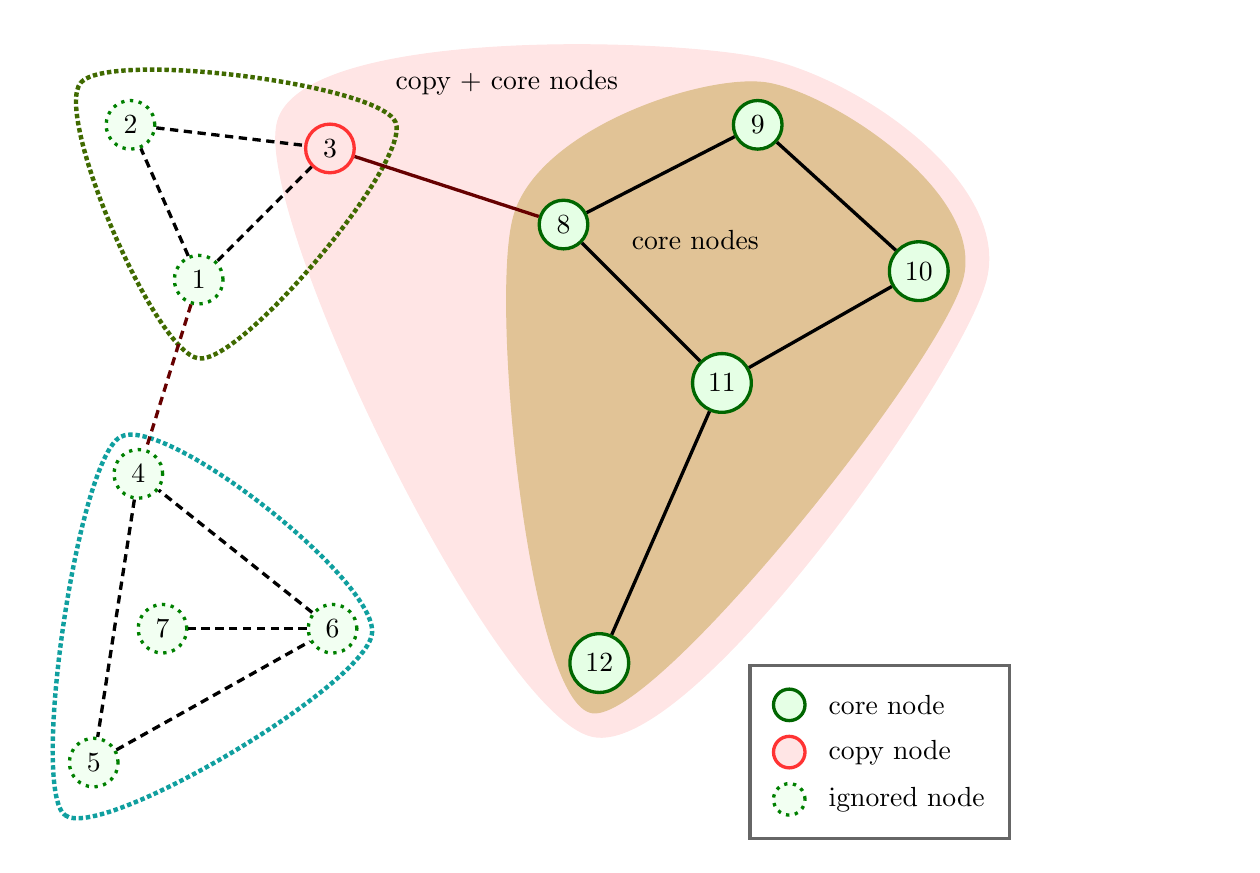
\begin{tikzpicture}[
        core_node/.style={circle, draw=black!60!green, fill=green!10,very thick, minimum size=4mm},
        copy_node/.style={circle, draw=red!80, fill=red!10, very thick, minimum size=4mm},
        core_node_ignore/.style={circle, dotted, draw=black!50!green, fill=green!5,very thick, minimum size=4mm}
        ]
            % Areas
            % rgb:pink,10;green,2;yellow,1
            \filldraw [color=red!10] plot [mark=none, smooth cycle] coordinates { (1,2)  (7.2,2.8)  (10,0) (5, -5.8)};
            \draw [color={rgb:red,2;green,4;yellow,1;black,5}, ultra thick,  densely dotted] plot [mark=none, smooth cycle] coordinates {(0,-1)  (-1.5,2.5)  (2.5,2) };
            \draw[color={rgb:red,1;cyan,10;black,5}, ultra thick,  densely dotted] plot [mark=none, smooth cycle] coordinates {(-1,-2)  (-1.7,-6.8)  (2.2,-4.5) };
            \filldraw[color={rgb:red,4;green,2;yellow,1;white,10}] plot [mark=none, smooth cycle] coordinates {(4,0.8)  (7.2,2.5)  (9.7,0) (5, -5.5)};


            % transmission
            \node[core_node_ignore]    (core_1)                                               {1};
            \node[core_node_ignore]    (core_2)   [above left  = 15mm and 4mm of core_1]      {2};
            \node[copy_node]    (core_3)   [above right = 12mm and 12mm of core_1]     {3};
            % distribution 1
            \node[core_node_ignore]    (core_4)   [below left  = 20mm and 3mm of core_1]             {4};
            \node[core_node_ignore]    (core_5)   [below left  = 32mm and 1mm of core_4]      {5};
            \node[core_node_ignore]    (core_6)   [below right = 15mm and 20mm of core_4]     {6};
            \node[core_node_ignore]    (core_7)   [left        = 15mm of core_6]              {7};
            % distribution 2
            \node[core_node]    (core_8)   [below right  = 5mm and 25 mm of core_3]           {8};
            \node[core_node]    (core_9)   [above right  = 8mm and 20mm of core_8]     {9};
            \node[core_node]    (core_10)  [below right  = 0.8mm and 40mm of core_8]   {10};
            \node[core_node]    (core_11)  [below right  = 15mm and 15mm of core_8]    {11};
            \node[core_node]    (core_12)  [below left  = 30mm and 10mm of core_11]    {12};
            
            % Lines
            \draw[black, very thick, densely dashed] (core_1) -- (core_2);
            \draw[black, very thick, densely dashed] (core_2) -- (core_3);
            \draw[black, very thick, densely dashed] (core_3) -- (core_1);
            \draw[black, very thick, densely dashed] (core_4) -- (core_5);
            \draw[black, very thick, densely dashed] (core_5) -- (core_6);
            \draw[black, very thick, densely dashed] (core_6) -- (core_7);
            \draw[black, very thick, densely dashed] (core_6) -- (core_4);
            \draw[black, very thick] (core_8) -- (core_9);
            \draw[black, very thick] (core_9) -- (core_10);
            \draw[black, very thick] (core_10) -- (core_11);
            \draw[black, very thick] (core_11) -- (core_12);
            \draw[black, very thick] (core_11) -- (core_8);
            % connection
            \draw[color=black!60!red, very thick, densely dashed] (core_1) -- (core_4);
            \draw[color=black!60!red, very thick] (core_3) -- (core_8);
            
            % text
            \node[text width=5cm] at (5, 2.5) {copy + core nodes};
            \node[text width=5cm] at (8, 0.5) {core nodes};
            % grid to estimate coordinate
            % \draw[step=1cm,gray,very thin, -] (-2,-8) grid (10,4);
            % legend
            \draw[color = black!60, fill = white, very thick] (7cm,-4.9cm) rectangle (10.3cm,-7.1cm);
            \node[core_node] at (7.5cm,-5.4cm)        { };
            \node[copy_node] at (7.5cm,-6cm)        { };
            \node[core_node_ignore] at (7.5cm,-6.6cm) { };
            \node[text width=5cm] at (10.5cm,-5.4cm) {core node};
            \node[text width=5cm] at (10.5cm, -6cm) {copy node};
            \node[text width=5cm] at (10.5cm, -6.6cm) {ignored node};
        \end{tikzpicture}
    \end{figure}

\end{document}